%\title{LaTeX Portrait Poster Template}
%%%%%%%%%%%%%%%%%%%%%%%%%%%%%%%%%%%%%%%%%
% a0poster Portrait Poster
% LaTeX Template
% Version 1.0 (22/06/13)
%
% The a0poster class was created by:
% Gerlinde Kettl and Matthias Weiser (tex@kettl.de)
% 
% Adapter by Jens Buysse for Hogeschool Gent
% This template has been downloaded from:
% http://www.LaTeXTemplates.com
%
% License:
% CC BY-NC-SA 3.0 (http://creativecommons.org/licenses/by-nc-sa/3.0/)
%
%%%%%%%%%%%%%%%%%%%%%%%%%%%%%%%%%%%%%%%%%

%----------------------------------------------------------------------------------------
%	PACKAGES AND OTHER DOCUMENT CONFIGURATIONS
%----------------------------------------------------------------------------------------

\documentclass[a0,portrait]{a0poster}

\usepackage{multicol} % This is so we can have multiple columns of text side-by-side
\columnsep=100pt % This is the amount of white space between the columns in the poster
\columnseprule=3pt % This is the thickness of the black line between the columns in the poster

\usepackage[svgnames]{xcolor} % Specify colors by their 'svgnames', for a full list of all colors available see here: http://www.latextemplates.com/svgnames-colors

\usepackage{times} % Use the times font
%\usepackage{palatino} % Uncomment to use the Palatino font

\usepackage{graphicx} % Required for including images
\graphicspath{{figures/}} % Location of the graphics files
\usepackage{booktabs} % Top and bottom rules for table
\usepackage[font=small,labelfont=bf]{caption} % Required for specifying captions to tables and figures
\usepackage{amsfonts, amsmath, amsthm, amssymb} % For math fonts, symbols and environments
\usepackage{wrapfig} % Allows wrapping text around tables and figures
\usepackage[export]{adjustbox}

\begin{document}

%----------------------------------------------------------------------------------------
%	POSTER HEADER 
%----------------------------------------------------------------------------------------

% The header is divided into two boxes:
% The first is 75% wide and houses the title, subtitle, names, university/organization and contact information
% The second is 25% wide and houses a logo for your university/organization or a photo of you
% The widths of these boxes can be easily edited to accommodate your content as you see fit

\begin{minipage}[t]{0.75\linewidth}
\VeryHuge \color{HoGentAccent1} \textbf{Het nut van pre-trained machine learning API’s voor het classificeren van foto-archieven} \color{Black}\\ % Title
\Huge\textit{Een vergelijkende studie tussen Google Vision, AWS Rekognition en imagga}\\[2.4cm] % Subtitle
\huge \textbf{Van Ruyskensvelde Frederik, Devos Timon, Dekoning Guy}\\[0.5cm] % Author(s)
\huge Hogeschool Gent, Valentin Vaerwyckweg 1, 9000 Gent\\[0.4cm] % University/organization
\Large \texttt{frederik.vanruyskensvelde@hogent.be} \\
\end{minipage}
%
\begin{minipage}[t]{0.25\linewidth}

\includegraphics[width=13cm,right]{figures/HOGENT_Logo_Pos_rgb.png} 

\end{minipage}

\vspace{1cm} % A bit of extra whitespace between the header and poster content

%----------------------------------------------------------------------------------------

\begin{multicols}{2} % This is how many columns your poster will be broken into, a portrait poster is generally split into 2 columns

%----------------------------------------------------------------------------------------
%	ABSTRACT
%----------------------------------------------------------------------------------------

\color{HoGentAccent1} % Navy color for the abstract

\begin{abstract}
Computer vision is een veld in AI en wordt gebruikt om computers te laten ''zien''. In deze studie wordt onderzocht of computer vision gebruikt kan worden voor het labelen van foto-archieven aan de hand van 3 verschillende organisaties die computer vision aanbieden via een API. De organisaties achter deze API's zijn Google Vision, AWS Rekognition en imagga. Uit het onderzoek blijkt dat Google Vision en AWS Rekognition nuttig kunnen zijn bij het labelen van foto-archieven, ze kunnen echter geen mensen vervangen en kunnen als hulpmiddel aanzien worden.
\end{abstract}
%----------------------------------------------------------------------------------------
%	INTRODUCTION
%----------------------------------------------------------------------------------------

\color{HoGentAccent1} 
\section*{Introductie}
\color{black}
\color{black}
Machine learning en AI (Artificiële Intelligentie) heeft het laatste decennium een sprong voorwaarts gemaakt. Sinds de opkomst van cloud computing kiezen steeds meer bedrijven voor de implementatie van een vorm van AI.

Op basis van deze evolutie leek het interessant om te onderzoeken of AI en machine learning kan toegepast worden op een concrete business case. Er zijn veel organisaties die grote foto-archieven hebben, zowel fysiek als digitaal, waarop niet gezocht kan worden. Het manueel zoekbaar maken van de foto-archieven is typisch een tijdrovend en vervelend werk, het automatiseren van dit proces zou voor grote tijdswinsten kunnen zorgen. Deze studie vergelijkt de resultaten van 3 verschillende computer vision providors bij het automatisch zoekbaar maken van archief-foto's. Er werd gekozen om enkel met computer vision providers te werken die een API aanbieden om de technische instap voor bedrijven zo klein mogelijk te houden.
%----------------------------------------------------------------------------------------
%	GEOLOGY
%----------------------------------------------------------------------------------------

\color{Black} % DarkSlateGray color for the rest of the content
\color{HoGentAccent1} 
\section*{Experimenten}
\color{black}
Om een realistisch experiment uit te voeren werd er via de Beeldbank van Archief Gent een dataset van 30 archief-foto's bekomen. De dataset bestaat uit foto's uit verschillende tijdsperiodes, van 1900 tot 2020.

Deze foto's werden via een custom dotnet applicatie aan de 3 verschillende API's aangeboden, iedere API retourneerde voor iedere foto 3 labels (labels zijn zowel objecten op de foto als meer abstracte concepten) en bij iedere label een zekerheidsgraad. Alle resultaten werden via de dotnet applicatie naar een csv geschreven. Ieder geretourneerd label werd handmatig gescoord, van 'volledig correct' tot 'niet correct'. De scores werden voor iedere API vergeleken, er werd ook rekening gehouden met de zekerheidsgraad; alle labels met een zekerheidsgraad onder een bepaalde threshold - in dit onderzoek, \char`75\% -  werden in een aparte categorie ingedeeld.

\color{HoGentAccent1} 
\section*{Sectie met figuur}
\color{black}


\begin{center}\vspace{1cm}
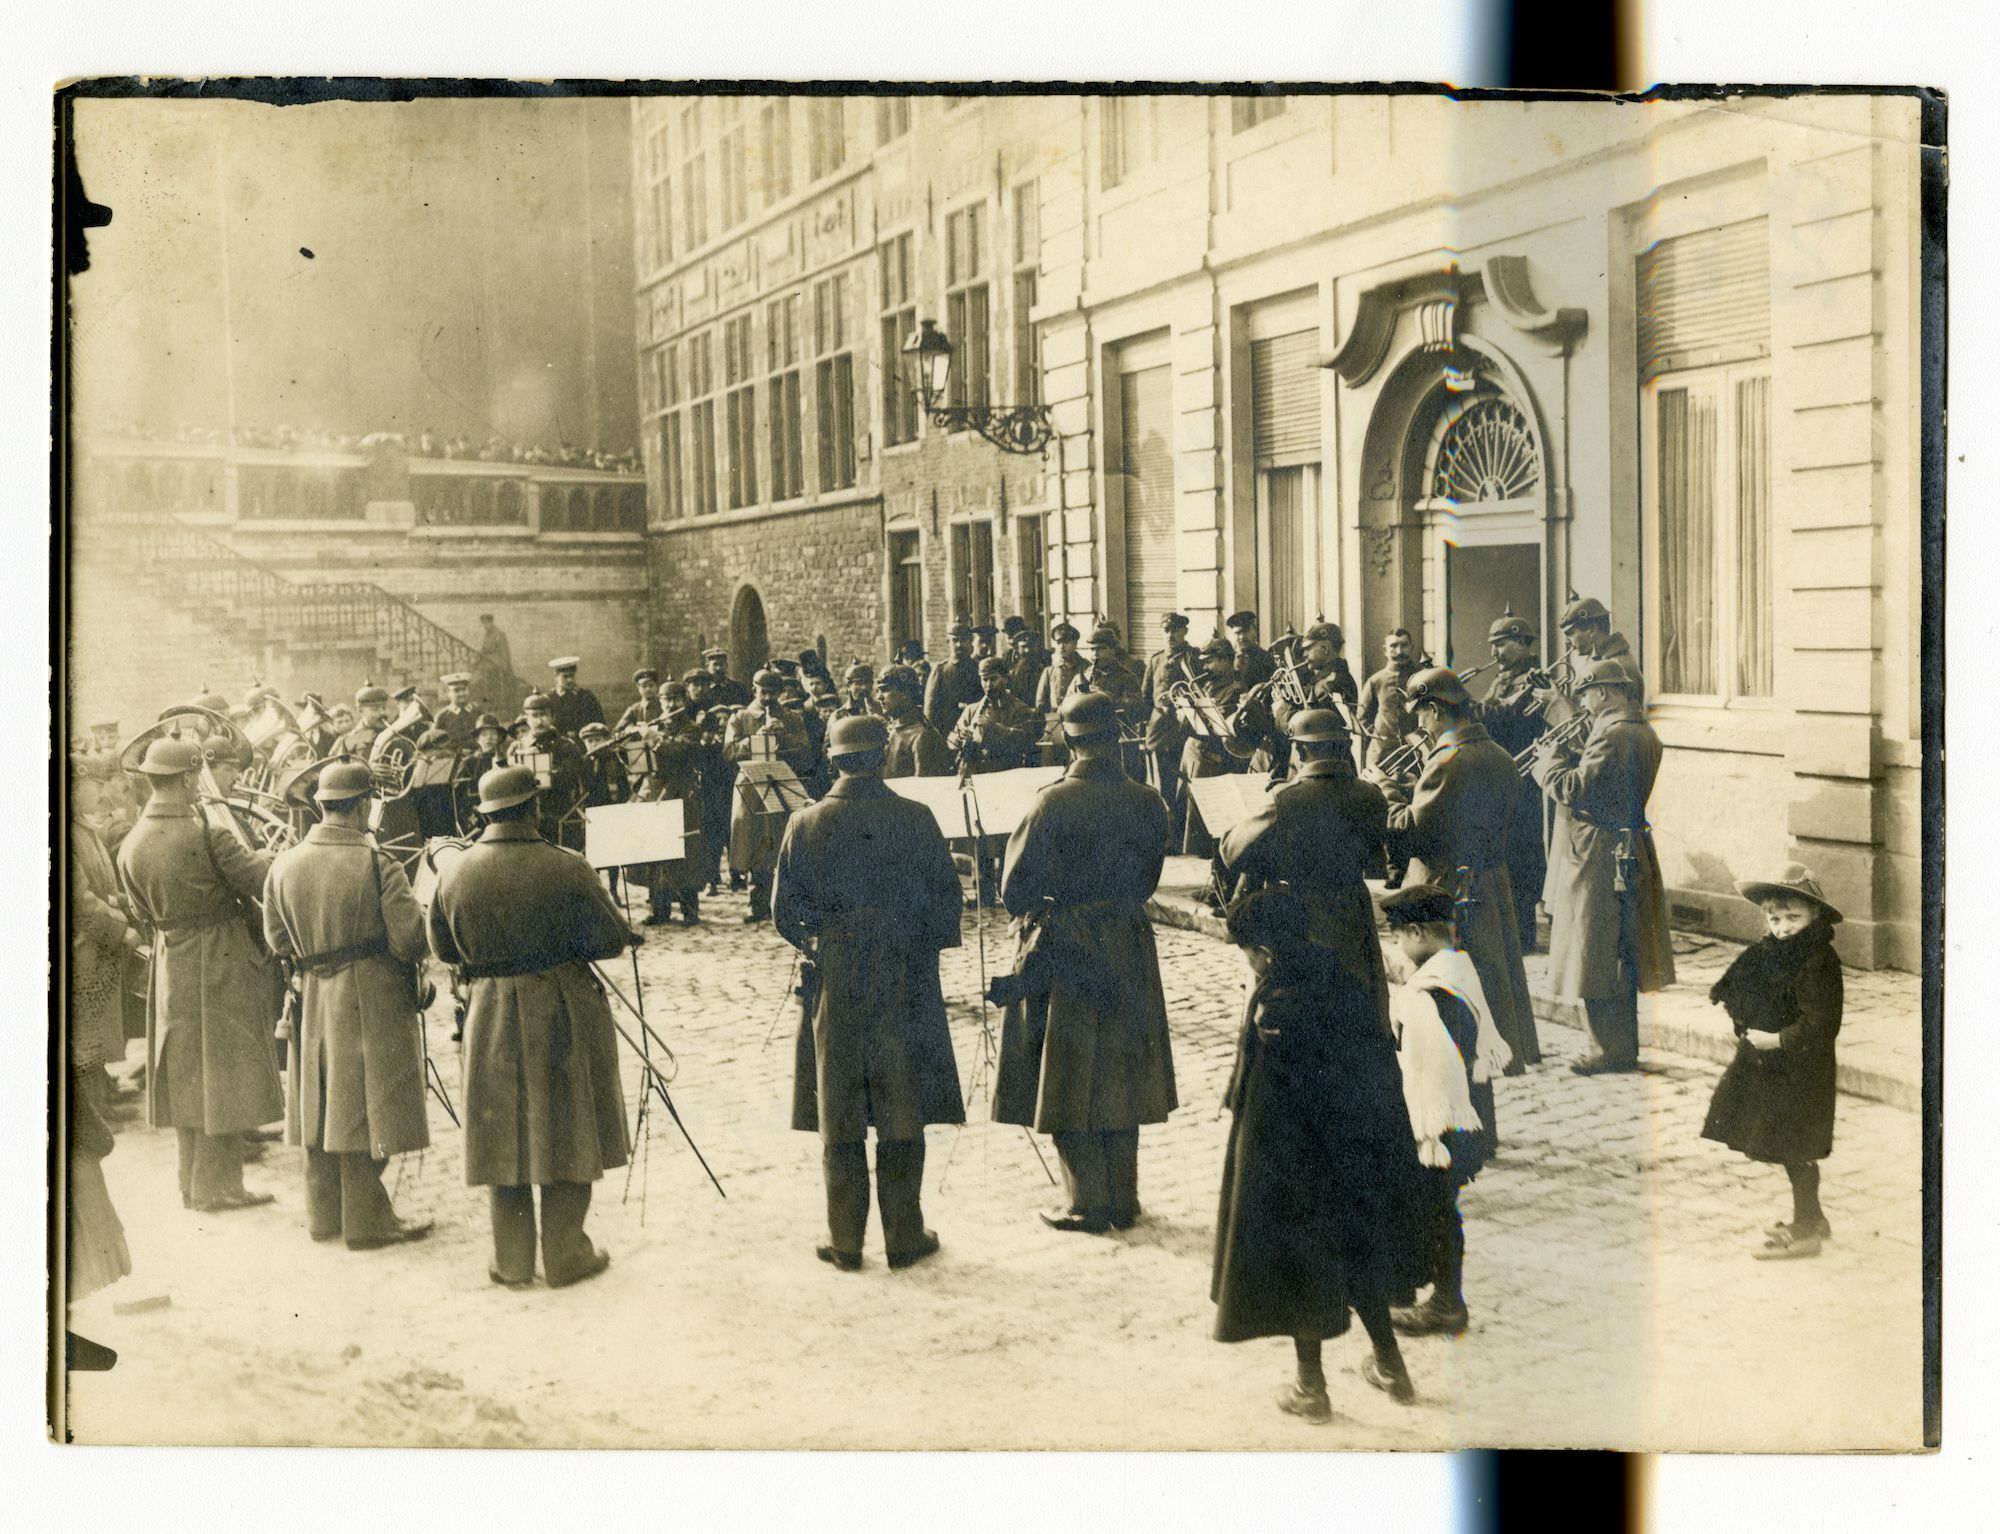
\includegraphics[width=1.0\linewidth]{sample28}
\captionof{figure}{\color{HoGentAccent5} Sample28 uit de dataset. Gevonden labels per API met zekerheidsgraad:
    Google Vision: Building 86\%, Art 82\%, Vintage Clothing 74\%;
    AWS Rekognition: Person 99\%, People 82\%, Funeral 74\%;
    imagga: brass 29\%, wind instrument 29\%, musical instrument 24\%.
Bron foto: ''Gent: Korenlei en Sint-Michielsbrug: concert door een militaire muziekkapel voor de verjaardag van de Duitse keizer Wilhelm II, 27 januari 1916'' - Beeldbank, Archief Gent (https://beeldbank.stad.gent/index.php)}
\end{center}\vspace{1cm}

%------------------------------------------------

\color{HoGentAccent1} 
\section*{Conclusies}
\color{black}
Zowel Google Vision als AWS Rekognition kunnen gebruikt worden om foto's te labelen in een concrete business setting. imagga, de kleinste speler, scoorde niet hoog genoeg om bruikbaar te zijn. 

De setup en configuratie is minimaal en kan door een gemiddeld bedrijf opgezet worden. Idealiter wordt er een front-end rond een of meerdere van deze API’s gebouwd en kan een gewone PC gebruiker automatische labeling laten uitvoeren.

De labeling door API's heeft een hoge mate van correctheid (\char`\~ 90\%), toch schieten de API's momenteel op 1 vlak duidelijk te kort: het ontbreken van context. Context zorgt er voor dat een persoon aan de hand van de volledige informatie vervat in de afbeelding kan inschatten welke labels er toepasbaar zijn. De computer vision API's ontbreken deze context volledig en geven bijgevolg regelmatig labels die te algemeen zijn en weinig waarde toevoegen. Het is dan ook belangrijk om te benadrukken dat de API's besproken in deze studie manuele labeling niet kan vervangen, het is interessanter om ze als een hulpmiddel te zien die archivarissen kunnen helpen om foto's sneller te labelen.
%----------------------------------------------------------------------------------------
%	FORTHCOMING RESEARCH
%----------------------------------------------------------------------------------------
\color{HoGentAccent1} 
\section*{Toekomstig onderzoek}
\color{black}
Het laatste decennium heeft computer vision op korte tijd veel vooruitgang geboekt, het zou dan ook interessant om een soortgelijk onderzoek opnieuw uit te voeren binnen 5 à 10 jaar en de resultaten te vergelijken. Verder onderzoek kan zich ook focussen op het dieper onderzoeken van de zekerheidsgraad threshold; welke threshold zorgt er voor de hoogste scores per API.


%----------------------------------------------------------------------------------------

\end{multicols}
\end{document}